\section{Definition of Measured Observables}
\label{sec:Obs}

The primary results of this thesis are the unfolded differential cross-sections of the following eleven different kinematic observables:

\begin{itemize}

\item{	$m_{4\ell}$: invariant mass of the four-lepton system (or $2$ $Z$-bosons)}
\item{ 	$m_{jj}$:  invariant mass of the dijet system}
\item{	$p_{T,4\ell}$: transverse momentum of the four-lepton system }
\item{	$p_{T, jj}$: transverse momentum of the dijet system}
\item{	$p_{T,4\ell jj}$: transverse momentum of the four-leptons and the dijet system}
\item{	$s_{T,4\ell jj}$: scalar transverse momentum of the four-leptons and the dijet system}
\item{ 	$\Delta \phi _{jj}^{signed}$: difference in the azimuthal angle between the two jets, ordered according to their rapidity, i.e. 
\begin{align*}
	\Delta \phi _{jj}^{signed} = 
	\begin{cases}
	\phi(j_1)-\phi(j_2) & \text{if $y_{j_1} > y_{j_2}$}\\
	\phi(j_2)-\phi(j_1) & \text{otherwise.}
	\end{cases} 
\end{align*}
}
\item{ $\Delta y_{jj}$: the absolute value of rapidity difference between the leading and the sub-leading jets}
\item{ $\zeta$: centrality of the system}
\item{ $\cos \theta^{*}_{\ell 1 \ell 2}$: cosine of the decay angle of the negative lepton of the leading pair in the pair's rest frame as shown by Figure \ref{fig:costhetaFrameOfRef}.}
\item{ $\cos \theta^{*}_{\ell 3 \ell 4}$: cosine of the decay angle of the negative lepton of the sub-leading pair in the pair's rest frame as shown by Figure \ref{fig:costhetaFrameOfRef}. }

\end{itemize}

\begin{figure}[!htb]
\centering
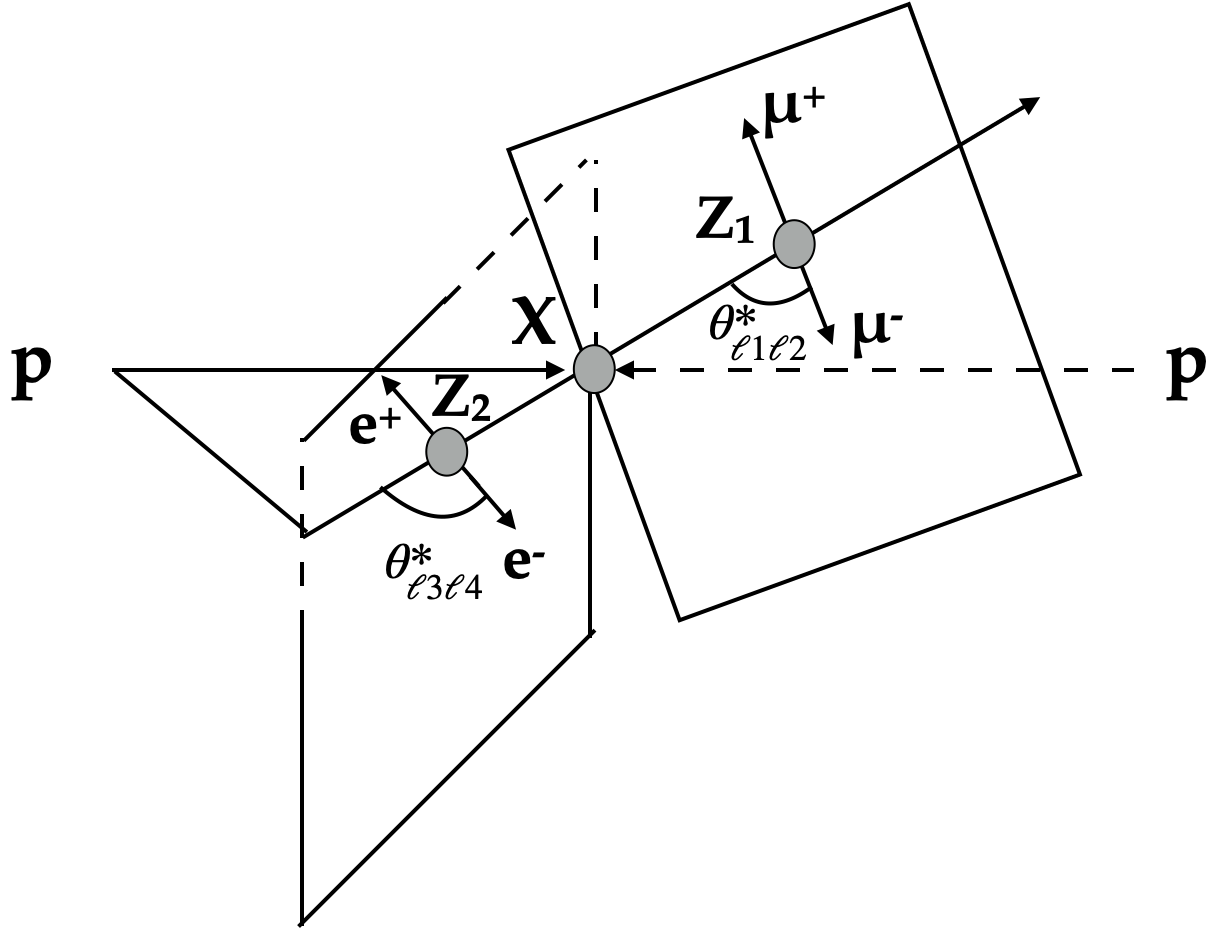
\includegraphics[width=.8\linewidth]{figures/AnalysisOverview/costhetaFrameOfRef.png}
\caption{Figure showing the decay angle $\theta^{*}_{\ell 1 \ell 2}$ ( $\theta^{*}_{\ell 3 \ell 4}$ ) of the negative lepton in the primary (secondary) pair's rest frame.\label{fig:costhetaFrameOfRef}\cite{AngularFrameDef}.}
\end{figure}
